\chapter{Estado del arte \label{cap:EstadoDelArte}}

La detección automatizada de noticias falsas ha emergido como una de las preocupaciones más apremiantes en la sociedad digital contemporánea, convirtiéndose en un campo de investigación multidisciplinario que abarca desde la ciencia de la computación hasta la psicología cognitiva. Durante la última década, investigadores de múltiples disciplinas han desarrollado enfoques innovadores que van desde técnicas tradicionales de procesamiento de lenguaje natural hasta modelos de lenguaje pre-entrenados de última generación, respondiendo a la creciente sofisticación de las campañas de desinformación y la velocidad sin precedentes con la que se propagan en las redes sociales.

En el contexto hispanohablante, esta problemática adquiere características particulares debido a las especificidades lingüísticas y culturales del español, incluyendo variaciones regionales, modismos locales, y patrones discursivos específicos que requieren enfoques metodológicos adaptados. La complejidad del español, con sus múltiples variantes geográficas y sus ricas estructuras sintácticas, presenta desafíos únicos para los sistemas automatizados de detección que tradicionalmente han sido desarrollados y entrenados principalmente en inglés.

Este capítulo examina de manera crítica las principales contribuciones científicas en el campo de la detección de desinformación, con especial énfasis en las aproximaciones que combinan técnicas de optimización metaheurística con modelos de aprendizaje automático. Se analiza también la evolución de los enfoques metodológicos, desde los primeros sistemas basados en características lingüísticas superficiales hasta los desarrollos más recientes que incorporan arquitecturas transformer y algoritmos de optimización bioinspirados, proporcionando un marco comprehensivo para entender tanto los avances logrados como los desafíos pendientes en este campo dinámico.

\section{Metodología de Búsqueda Bibliográfica}
\label{sec:busqueda_literatura}

Para garantizar una revisión comprehensiva y actualizada de la literatura científica en el campo de la detección de noticias falsas, se diseñó una estrategia de búsqueda sistemática que abarcó múltiples fuentes académicas reconocidas internacionalmente. Esta metodología se fundamentó en las mejores prácticas establecidas para revisiones sistemáticas de literatura en ciencias de la computación, siguiendo las directrices PRISMA adaptadas para el dominio tecnológico.

Las bases de datos consultadas incluyeron repositorios académicos de primer nivel como Google Scholar, Semantic Scholar, Nature Digital Libraries, IOPscience, MDPI, Web of Science (WoS) y repositorios especializados como arXiv. La selección de estas fuentes se basó en su cobertura disciplinaria, calidad editorial, y relevancia específica para el campo de procesamiento de lenguaje natural y detección de desinformación. Adicionalmente, se incluyeron conferencias especializadas como ACL, EMNLP, y talleres específicos como CheckThat! para capturar los desarrollos más recientes en el área.

La búsqueda se estructuró en torno a combinaciones específicas de términos que reflejan las dimensiones principales de esta investigación, utilizando operadores booleanos y comodines para maximizar la exhaustividad:

\begin{itemize}
    \item \textit{Spanish fake news detection} -- para capturar trabajos específicos del idioma español, incluyendo variaciones como "detección de noticias falsas en español"
    \item \textit{Fake news detection language models} -- para incluir enfoques basados en modelos de lenguaje, cubriendo términos como BERT, RoBERTa, y transformer
    \item \textit{Metaheuristic hyperparameter optimization} -- para identificar aplicaciones de optimización metaheurística en aprendizaje automático
    \item \textit{Employment fraud detection} -- para abarcar el dominio del fraude laboral y su detección automatizada
    \item \textit{Simulated annealing fake news} y \textit{Genetic algorithm text classification} -- para enfoques específicos de optimización aplicados a clasificación textual
    \item \textit{Social media misinformation detection} -- para capturar trabajos enfocados en plataformas sociales
    \item \textit{Cross-lingual fake news} y \textit{multilingual misinformation} -- para incluir enfoques multilingües
\end{itemize}

El proceso de selección aplicó criterios rigurosos de relevancia temática, calidad metodológica y actualidad temporal. Se priorizaron publicaciones de los últimos cinco años (2019-2024) sin excluir trabajos seminales fundamentales para el campo que, aunque anteriores, establecieron bases teóricas o metodológicas esenciales. Los criterios de inclusión incluyeron: (1) contribuciones metodológicas originales, (2) validación empírica robusta, (3) relevancia directa para la detección de desinformación, y (4) calidad de la revisión por pares. Los criterios de exclusión abarcaron: (1) trabajos puramente teóricos sin validación, (2) estudios con muestras insuficientes, (3) publicaciones en idiomas distintos al inglés o español, y (4) trabajos duplicados o versiones preliminares de conferencias posteriormente publicadas en revistas.

Como resultado de este proceso sistemático y riguroso, se identificaron 76 trabajos que constituyen el núcleo de esta revisión, organizados temáticamente para facilitar el análisis comparativo y la identificación de tendencias emergentes en el campo.

\section{Panorama de la Investigación en Detección de Noticias Falsas}
\label{sec:panorama_investigacion}

El campo de la detección automatizada de desinformación ha experimentado una evolución notable y acelerada, caracterizada por una transición paradigmática desde enfoques tradicionales basados en características estadísticas simples hacia sistemas sofisticados que integran múltiples modalidades, técnicas de optimización avanzadas, y conocimiento contextual profundo. Esta evolución refleja tanto los avances tecnológicos en inteligencia artificial como la creciente sofisticación de las técnicas de desinformación empleadas por actores maliciosos.

La progresión temporal del campo puede dividirse en tres fases principales: (1) la era pioneera (2010-2016), caracterizada por enfoques basados en características lingüísticas superficiales y métodos de aprendizaje automático tradicionales; (2) la era de los modelos profundos (2017-2020), marcada por la adopción masiva de redes neuronales profundas y arquitecturas transformer; y (3) la era contemporánea (2021-presente), dominada por modelos de lenguaje de gran escala y enfoques híbridos que combinan múltiples técnicas de optimización.

\subsection{Fundamentos Metodológicos y Construcción de Corpus}

La disponibilidad de conjuntos de datos de alta calidad constituye el fundamento sobre el cual se construye cualquier sistema de detección eficaz, y representa uno de los mayores desafíos en el desarrollo de tecnologías de detección de desinformación. En el contexto hispanohablante, esta necesidad se vuelve particularmente crítica debido a la relativa escasez de recursos comparado con el inglés, donde la mayoría de la investigación se ha concentrado históricamente.

Los trabajos pioneros en esta dirección han establecido las bases metodológicas para la construcción y evaluación de corpus especializados, desarrollando protocolos de anotación, criterios de calidad, y marcos de evaluación que han influido significativamente en el desarrollo del campo. Acosta \cite{acosta2019construccion} desarrolló uno de los primeros marcos sistemáticos para la construcción de conjuntos de datos de noticias en español, estableciendo criterios rigurosos de calidad y protocolos de etiquetado manual que han influido significativamente en trabajos posteriores. Su metodología, centrada en la extracción automatizada seguida de verificación manual exhaustiva, demostró la viabilidad de crear recursos lingüísticos de gran escala para el español mientras mantenía estándares de calidad comparables a los corpus en inglés. El trabajo incluye un análisis detallado de las fuentes de noticias, criterios de selección temporal, y metodologías de validación cruzada entre anotadores.

El trabajo seminal de Posadas-Durán et al. \cite{posadas2019detection} complementó estos esfuerzos al proponer un nuevo corpus específicamente diseñado para la detección de noticias falsas en español, incorporando características estilométricas innovadoras que capturan patrones lingüísticos sutiles pero significativos para la identificación de contenido desinformativo. Este enfoque pionero en el análisis del estilo de escritura como indicador de veracidad abrió nuevas líneas de investigación que han sido extensamente exploradas en trabajos posteriores. Su corpus incluye anotaciones multinivel que abarcan desde características superficiales del texto hasta análisis semánticos profundos, proporcionando un recurso invaluable para investigaciones subsequentes.

La comunidad científica internacional ha reconocido la importancia crítica de esta área a través de iniciativas competitivas sistemáticas que han proporcionado marcos estandarizados para la evaluación y comparación de sistemas. Los talleres CheckThat! organizados en el marco de CLEF \cite{alam2023overview, barron2023clef} han proporcionado marcos estandarizados para la evaluación comparativa de sistemas de detección, estableciendo métricas unificadas, protocolos de evaluación rigurosos, y conjuntos de datos de referencia que han contribuido significativamente a la maduración metodológica del campo. Estos talleres han evolucionado para incluir tareas cada vez más sofisticadas, desde la verificación de hechos básica hasta la detección de sesgo político y la evaluación de credibilidad en contenido multimodal.

\textbf{Un desafío fundamental en este campo es que no todos los corpus disponibles son equivalentes en términos de propósito, metodología de construcción, o calidad de anotación}. Esta heterogeneidad refleja la evolución natural del campo, donde diferentes grupos de investigación han abordado aspectos específicos del problema con enfoques metodológicos diversos. Algunos corpus se enfocan en análisis estilométrico, otros en detección política, y otros en evaluación de modelos específicos, lo que genera un ecosistema rico pero complejo de recursos disponibles.

En el contexto iberoamericano específicamente, las competiciones IberLEF han jugado un papel fundamental en el desarrollo de recursos y metodologías adaptadas a las particularidades del español. Aragón et al. \cite{aragon2020overview} documentaron los primeros esfuerzos sistemáticos para abordar la detección de noticias falsas en español mexicano, estableciendo benchmarks específicos para variantes regionales del idioma y desarrollando métricas de evaluación culturalmente sensibles. Paralelamente, Gómez-Adorno et al. \cite{gomez2021overview} consolidaron estos esfuerzos en el marco de FakeDeS, estableciendo un referente duradero para la evaluación de sistemas en español que incluye tanto aspectos técnicos como consideraciones socioculturales.

La evolución hacia recursos más sofisticados y comprehensivos se refleja en iniciativas recientes como el Spanish Fake News Corpus Version 2.0 \cite{ramirez2021spanish}, que incorpora anotaciones multinivel y metadatos enriquecidos que permiten análisis más profundos y matizados de los patrones de desinformación. Este corpus de segunda generación incluye información contextual sobre fuentes, temas, y patrones temporales de propagación, proporcionando un recurso sin precedentes para la investigación en detección automatizada.

\begin{table}[htbp]
\centering
\adjustbox{width=\textwidth,center}{%
\small
\begin{tabular}{|l|l|l|c|c|}
\hline
\rowcolor{UAMPurple!20}
\textbf{Contribución Principal} & \textbf{Autores} & \textbf{Publicación} & \textbf{Año} & \textbf{Ref.} \\
\hline
\begin{tabular}[t]{@{}l@{}}Marco metodológico para construcción\\de conjuntos de datos de noticias en español\end{tabular} & Acosta, F. A. Z. & U. Politécnica de Madrid & 2019 & \cite{acosta2019construccion} \\
\hline
\begin{tabular}[t]{@{}l@{}}Evaluación multimodal y multigenre\\para verificación de contenido\end{tabular} & Alam, F., et al. & CEUR Workshop Proc. & 2023 & \cite{alam2023overview} \\
\hline
\begin{tabular}[t]{@{}l@{}}Análisis de agresividad y desinformación\\en español mexicano\end{tabular} & Aragón, M. E., et al. & IberLEF Workshop & 2020 & \cite{aragon2020overview} \\
\hline
\begin{tabular}[t]{@{}l@{}}Marco estandardizado CheckThat!\\para evaluación de sistemas\end{tabular} & Barrón-Cedeño, A., et al. & ECIR 2023 & 2023 & \cite{barron2023clef} \\
\hline
\begin{tabular}[t]{@{}l@{}}Consolidación de métricas FakeDeS\\para detección en español\end{tabular} & Gómez-Adorno, H., et al. & Procesamiento del Lenguaje Natural & 2021 & \cite{gomez2021overview} \\
\hline
\begin{tabular}[t]{@{}l@{}}Corpus pionero con características\\estilométricas para español\end{tabular} & Posadas-Durán, J. P., et al. & J. of Intelligent and Fuzzy Systems & 2019 & \cite{posadas2019detection} \\
\hline
\begin{tabular}[t]{@{}l@{}}Corpus enriquecido con anotaciones\\multinivel versión 2.0\end{tabular} & Ramírez Cruz, J. M., et al. & GitHub Repository & 2021 & \cite{ramirez2021spanish} \\
\hline
\begin{tabular}[t]{@{}l@{}}Técnicas de aprendizaje automático\\aplicadas al español\end{tabular} & Tretiakov, A., et al. & Springer & 2022 & \cite{tretiakov2022detection} \\
\hline
\end{tabular}
}
\caption{Contribuciones fundamentales en metodología y construcción de corpus para español.}
\label{tab:articulos_metodologia}
\end{table}

Esta base metodológica sólida y en constante evolución ha permitido el desarrollo de aproximaciones cada vez más sofisticadas que integran múltiples tipos de evidencia, técnicas de análisis avanzadas, y conocimiento contextual, estableciendo el terreno fértil para los desarrollos contemporáneos en modelos de lenguaje de gran escala y optimización metaheurística que se analizan en las siguientes secciones.

\subsection{Evolución de los Modelos de Lenguaje en Detección de Desinformación}

La irrupción de los modelos de lenguaje pre-entrenados ha revolucionado completamente el panorama de la detección automatizada de noticias falsas, representando un cambio paradigmático fundamental en cómo conceptualizamos y abordamos la comprensión automatizada de texto. Esta transformación se caracteriza por una progresión clara y acelerada desde arquitecturas básicas hacia sistemas cada vez más sofisticados que integran conocimiento contextual profundo, capacidades de razonamiento complejo, y comprensión semántica avanzada.

El punto de inflexión histórico llegó con la introducción de BERT \cite{devlin2018bert}, cuya arquitectura bidireccional revolucionaria permitió capturar dependencias contextuales de manera más efectiva y matizada que los enfoques secuenciales previos basados en LSTM o GRU. La capacidad fundamental de BERT para entender el contexto completo de una oración de manera simultánea, en lugar de procesarla secuencialmente de izquierda a derecha como los modelos anteriores, representó un avance fundamental que ha sido extensamente aplicado y adaptado en la detección de desinformación. Esta arquitectura bidireccional permite al modelo capturar relaciones complejas entre palabras que pueden estar distantes en el texto pero semánticamente relacionadas, una característica crucial para identificar inconsistencias sutiles y patrones desinformativos sofisticados.

La necesidad imperativa de modelos más eficientes computacionalmente, especialmente para aplicaciones en tiempo real y dispositivos con recursos limitados, llevó al desarrollo de variantes optimizadas como DistilBERT \cite{sanh2019distilbert}, que mantiene aproximadamente el 97% del rendimiento de BERT con solo el 60% de sus parámetros mediante técnicas innovadoras de destilación de conocimiento. Esta línea de investigación, que incluye también desarrollos como TinyBERT \cite{jiao2019tinybert}, ha demostrado ser crucial para aplicaciones prácticas de detección en tiempo real donde los recursos computacionales son limitados pero la precisión no puede comprometerse significativamente.

En el contexto específico y culturalmente relevante del español, el trabajo comprehensivo de Martínez-Gallego et al. \cite{martinez2021fake} exploró sistemáticamente la aplicación de técnicas de aprendizaje profundo, incluyendo tanto BERT como BETO (la variante específicamente pre-entrenada en español), para la detección de noticias falsas. Sus resultados empíricos demostraron de manera convincente que los modelos específicamente pre-entrenados en español superan consistentemente a las versiones multilingües genéricas, subrayando la importancia crítica de la especialización lingüística y cultural en el desarrollo de sistemas de detección efectivos. Este hallazgo tiene implicaciones profundas para el desarrollo de sistemas de detección en idiomas distintos al inglés.

Blanco-Fernández et al. \cite{blanco2024enhancing} extendieron significativamente esta línea de investigación al comparar sistemáticamente BERT y RoBERTa en tareas específicas de detección de desinformación en español, proporcionando evidencia empírica detallada sobre las ventajas relativas de diferentes arquitecturas transformer para este dominio específico. Su trabajo demostró que RoBERTa, con su entrenamiento más extenso y metodología de enmascaramiento optimizada, puede ofrecer mejoras significativas en la detección de patrones sutiles de desinformación, especialmente en textos que emplean técnicas de manipulación sofisticadas.

El surgimiento explosivo de modelos generativos de gran escala ha introducido dimensiones completamente nuevas y complejas al problema de detección. Brown et al. \cite{brown2020language} establecieron con GPT-3 las bases conceptuales y técnicas de los modelos de lenguaje de gran escala, cuyas capacidades avanzadas de generación de texto han complicado paradójicamente el problema de detección al crear contenido sintético cada vez más indistinguible del contenido humano auténtico. El equipo de Gemini \cite{gemini2023family} ha continuado esta evolución hacia modelos multimodales que pueden procesar y generar simultáneamente texto, imágenes y otros tipos de información, ampliando el alcance y la complejidad de los desafíos de detección.

Esta evolución acelerada ha generado nuevos desafíos metodológicos y éticos que requieren enfoques innovadores. Su et al. \cite{su2023adapting} analizaron cómo la era de los modelos de lenguaje grandes requiere adaptaciones fundamentales en las técnicas de detección tradicionales, incluyendo nuevos marcos teóricos y metodológicos para abordar contenido generado artificialmente. Complementariamente, su trabajo posterior \cite{su2023fake} reveló que los detectores existentes muestran sesgos sistemáticos significativos contra texto generado por LLMs, planteando cuestiones fundamentales sobre la generalización, robustez, y equidad de los sistemas de detección contemporáneos.

El enfoque hacia la mejora continua y la adaptación de estos sistemas se refleja en trabajos innovadores como el de Shushkevich et al. \cite{shushkevich2023improving}, que exploraron la combinación sinérgica de modelos BERT con datos aumentados mediante ChatGPT, demostrando cómo los propios LLMs pueden utilizarse estratégicamente para mejorar la detección de contenido falso mediante técnicas de augmentación de datos y transferencia de conocimiento.

Una perspectiva particularmente interesante e importante emerge del trabajo de Hu et al. \cite{hu2024bad}, que examina el papel dual y paradójico de los modelos de lenguaje grandes como potenciales generadores de desinformación y, simultáneamente, como herramientas para su detección. Esta dualidad fundamental refleja la complejidad creciente del panorama tecnológico actual y plantea cuestiones éticas y prácticas importantes sobre el desarrollo responsable de tecnologías de IA.

\begin{table}[htbp]
\centering
\adjustbox{width=\textwidth,center}{%
\small
\begin{tabular}{|l|l|l|c|c|}
\hline
\rowcolor{UAMPurple!20}
\textbf{Innovación Principal} & \textbf{Autores} & \textbf{Publicación} & \textbf{Año} & \textbf{Ref.} \\
\hline
\begin{tabular}[t]{@{}l@{}}Arquitectura bidireccional para\\comprensión contextual profunda\end{tabular} & Devlin, J., et al. & arXiv & 2018 & \cite{devlin2018bert} \\
\hline
\begin{tabular}[t]{@{}l@{}}Destilación de conocimiento para\\modelos eficientes\end{tabular} & Sanh, V., et al. & arXiv & 2019 & \cite{sanh2019distilbert} \\
\hline
\begin{tabular}[t]{@{}l@{}}Optimización extrema con\\TinyBERT\end{tabular} & Jiao, X., et al. & arXiv & 2019 & \cite{jiao2019tinybert} \\
\hline
\begin{tabular}[t]{@{}l@{}}Aplicación sistemática de transformers\\en español\end{tabular} & Martínez-Gallego, K., et al. & arXiv & 2021 & \cite{martinez2021fake} \\
\hline
\begin{tabular}[t]{@{}l@{}}Comparación BERT vs RoBERTa\\para español\end{tabular} & Blanco-Fernández, Y., et al. & Applied Sciences & 2024 & \cite{blanco2024enhancing} \\
\hline
\begin{tabular}[t]{@{}l@{}}Capacidades emergentes en\\modelos de gran escala\end{tabular} & Brown, T. B., et al. & arXiv & 2020 & \cite{brown2020language} \\
\hline
\begin{tabular}[t]{@{}l@{}}Modelos multimodales de\\próxima generación\end{tabular} & Gemini Team, Google & arXiv & 2023 & \cite{gemini2023family} \\
\hline
\begin{tabular}[t]{@{}l@{}}Adaptación para la era\\de LLMs\end{tabular} & Su, J., et al. & arXiv & 2023 & \cite{su2023adapting} \\
\hline
\end{tabular}
}
\caption{Evolución de modelos de lenguaje aplicados a detección de desinformación.}
\label{tab:modelos_lenguaje}
\end{table}

\subsection{Técnicas de Optimización Metaheurística en Detección de Desinformación}

La aplicación sistemática de algoritmos metaheurísticos a la detección de noticias falsas representa una convergencia natural e innovadora entre dos áreas de investigación que han madurado de manera independiente pero complementaria durante las últimas décadas. Por un lado, las metaheurísticas han demostrado repetidamente su eficacia excepcional en la resolución de problemas de optimización complejos, no lineales, y multimodales en múltiples dominios científicos y de ingeniería. Por otro lado, la detección de desinformación enfrenta desafíos inherentes y crecientes de optimización, particularmente en la calibración precisa de hiperparámetros, la selección inteligente de características relevantes, y la optimización de arquitecturas de modelos complejos.

La formulación innovadora de la detección de noticias falsas como un problema de optimización combinatorial presenta ventajas significativas tanto desde perspectivas teóricas como prácticas. Esta reformulación permite la aplicación de décadas de investigación en optimización metaheurística a un problema social contemporáneo de gran relevancia. Aqil y Lahby \cite{aqil2021modeling} fueron pioneros visionarios en modelar esta tarea como un problema de planificación de tareas (Job Shop Scheduling), donde diferentes algoritmos de procesamiento de texto deben ejecutarse de manera óptima considerando restricciones de tiempo, recursos computacionales, y calidad de resultados. Su evaluación comparativa exhaustiva de tres metaheurísticas principales (Iterated Greedy, Algoritmos Genéticos y Artificial Bee Colony) demostró empíricamente que Iterated Greedy superaba consistentemente a las alternativas en términos tanto de eficiencia computacional como de calidad de soluciones, estableciendo un precedente metodológico importante para investigaciones posteriores.

En el ámbito específico y técnicamente desafiante de la detección de reseñas falsas, que comparte muchas características con la detección de noticias falsas, Deshai y Rao \cite{deshai2023unmasking} desarrollaron un enfoque innovador y técnicamente sofisticado que combina redes neuronales convolucionales (CNN) con Optimización por Enjambre de Partículas adaptativo (PSO). Su contribución principal radica en la demostración empírica y teórica de que PSO puede optimizar efectivamente los hiperparámetros complejos de redes CNN, superando métodos tradicionales como Grid Search y Random Search en términos de eficiencia computacional, convergencia, y calidad de resultados finales. El trabajo incluye un análisis detallado de la superficie de respuesta del espacio de hiperparámetros y demuestra cómo PSO puede navegar eficientemente estos espacios multidimensionales complejos.

El trabajo comprehensivo y metodológicamente riguroso de Bacanin et al. \cite{bacanin2023benefits} proporciona evidencia sistemática y estadísticamente robusta sobre los beneficios substantivos de utilizar metaheurísticas en la calibración de hiperparámetros de modelos de aprendizaje profundo. Aunque su enfoque primario se centra en predicción de cargas energéticas, sus hallazgos sobre la superioridad demonstrada de Algoritmos Genéticos Binarios, PSO y Recocido Simulado para optimizar modelos LSTM son directamente aplicables y transferibles al dominio de detección de texto y análisis de sentimientos. El estudio incluye análisis estadísticos exhaustivos, comparaciones con métodos baseline, y evaluaciones de significancia que proporcionan una base sólida para la adopción de estas técnicas en otros dominios.

Una perspectiva particularmente valiosa y metodológicamente innovadora emerge del trabajo de Das et al. \cite{das2022heuristic}, que desarrollaron un marco comprehensive basado en ensemble que integra técnicas heurísticas avanzadas para manejar la incertidumbre inherente y multifacética en la clasificación de tweets y artículos de noticias. Su enfoque reconoce explícitamente que la detección de desinformación no es simplemente un problema de clasificación binaria tradicional, sino que requiere el manejo sofisticado de múltiples fuentes de evidencia, grados de certidumbre variable, y contextos sociales complejos. El framework propuesto incluye mecanismos para cuantificar y propagar incertidumbre a través de múltiples etapas del pipeline de detección.

En el contexto culturalmente específico del hispanohablante, el trabajo pionero de Hurtado Avilés et al. \cite{hurtado2024calibracion} representa la primera aplicación sistemática y comprehensiva de metaheurísticas específicamente diseñada para la detección de fraude digital en español. Su contribución establece un marco metodológico robusto que integra múltiples algoritmos de optimización con modelos de lenguaje especializados, considerando las particularidades lingüísticas y culturales del español que afectan tanto la generación como la detección de contenido desinformativo.

La diversificación hacia enfoques híbridos y multimodales se ejemplifica brillantemente en el trabajo técnicamente avanzado de Yildirim \cite{yildirim2023novel}, que propone un enfoque multi-hilo novedoso que combina múltiples metaheurísticas para la detección multimodal de noticias falsas. Esta aproximación reconoce que los sistemas contemporáneos de desinformación integran sofisticadamente múltiples modalidades (texto, imágenes, videos, metadatos) que requieren estrategias de optimización coordinadas y sincronizadas para lograr detección efectiva en tiempo real.

\begin{table}[htbp]
\centering
\adjustbox{width=\textwidth,center}{%
\small
\begin{tabular}{|l|l|l|c|c|}
\hline
\rowcolor{UAMPurple!20}
\textbf{Contribución Metodológica} & \textbf{Autores} & \textbf{Publicación} & \textbf{Año} & \textbf{Ref.} \\
\hline
\begin{tabular}[t]{@{}l@{}}Formulación como problema de\\planificación de tareas\end{tabular} & Aqil, S., \& Lahby, M. & Studies in Comp. Intelligence & 2021 & \cite{aqil2021modeling} \\
\hline
\begin{tabular}[t]{@{}l@{}}PSO adaptativo para optimización\\de CNN en detección de reseñas\end{tabular} & Deshai, N., \& Rao, B. B. & Soft Computing & 2023 & \cite{deshai2023unmasking} \\
\hline
\begin{tabular}[t]{@{}l@{}}Evidencia sistemática de beneficios\\en modelos de aprendizaje profundo\end{tabular} & Bacanin, N., et al. & Energies & 2023 & \cite{bacanin2023benefits} \\
\hline
\begin{tabular}[t]{@{}l@{}}Marco ensemble para manejo\\de incertidumbre\end{tabular} & Das, S. D., et al. & Neurocomputing & 2022 & \cite{das2022heuristic} \\
\hline
\begin{tabular}[t]{@{}l@{}}Aplicación específica para\\español y fraude digital\end{tabular} & Hurtado Avilés, G., et al. & BUAP & 2024 & \cite{hurtado2024calibracion} \\
\hline
\begin{tabular}[t]{@{}l@{}}Enfoque multi-hilo para\\detección multimodal\end{tabular} & Yildirim, G. & Applied Intelligence & 2023 & \cite{yildirim2023novel} \\
\hline
\begin{tabular}[t]{@{}l@{}}Combinación K-Means y SVM\\para selección de características\end{tabular} & Yazdi, K. M., et al. & WASET & 2020 & \cite{yazdi2020improving} \\
\hline
\begin{tabular}[t]{@{}l@{}}Optimización de ensemble\\con metaheurísticas\end{tabular} & Yasmin, A., et al. & PLOS ONE & 2024 & \cite{yasmin2024ensemble} \\
\hline
\end{tabular}
}
\caption{Contribuciones metodológicas en optimización metaheurística para detección.}
\label{tab:articulos_metaheuristicas}
\end{table}

La diversificación creciente hacia enfoques híbridos se observa claramente en estudios metodológicamente innovadores como el de Yazdi et al. \cite{yazdi2020improving}, que combina técnicas de clustering K-Means con máquinas de vectores de soporte (SVM) para optimizar la selección de características en espacios de alta dimensionalidad. Su contribución demuestra empíricamente que la integración inteligente de metaheurísticas con técnicas de preprocesamiento puede mejorar significativamente la eficacia de detectores convencionales, especialmente en escenarios donde la dimensionalidad de los datos presenta desafíos computacionales significativos.

Finalmente, el trabajo técnicamente avanzado de Yasmin et al. \cite{yasmin2024ensemble} avanza decididamente hacia la optimización completa y sistemática de sistemas ensemble, donde múltiples metaheurísticas colaboran de manera coordinada en la calibración simultánea de pesos, hiperparámetros, y arquitecturas de diferentes clasificadores base. Este enfoque representa la frontera actual más avanzada en la aplicación de optimización metaheurística a problemas de detección complejos y establece precedentes importantes para desarrollos futuros en el campo.

\section{Algoritmos Metaheurísticos: Fundamentos Teóricos y Aplicaciones Prácticas}
\label{sec:algoritmos_metaheuristicos}

Los algoritmos metaheurísticos representan una clase fundamental y versátil de técnicas de optimización que han demostrado ser especialmente efectivas para resolver problemas complejos de optimización no lineal, no convexos, y multimodales, incluyendo específicamente la calibración de hiperparámetros en modelos de aprendizaje automático y la optimización de arquitecturas de redes neuronales. Esta sección presenta de manera comprehensiva los fundamentos teóricos, principios operativos, y aplicaciones prácticas de los principales algoritmos metaheurísticos utilizados en la detección de noticias falsas y optimización de modelos.

\subsection{Algoritmos Genéticos (GA): Evolución Artificial para Optimización}

Los Algoritmos Genéticos, introducidos originalmente por Holland \cite{holland1992adaptation} en su trabajo seminal sobre adaptación en sistemas naturales y artificiales, están inspirados profundamente en la teoría de la evolución de Darwin y los principios fundamentales de la genética molecular. Estos algoritmos mantienen una población diversa de soluciones candidatas que evolucionan iterativamente a través de operadores genéticos cuidadosamente diseñados como selección, cruzamiento (crossover), y mutación, mimando los procesos evolutivos naturales pero aplicados a espacios de soluciones abstractos.

El trabajo fundamental de Holland estableció no solo las bases teóricas para esta clase de algoritmos bioinspirados, sino también demostraciones formales de su capacidad para explorar eficientemente espacios de búsqueda complejos y multimodales mediante un balance inteligente entre exploración (búsqueda global) y explotación (refinamiento local). La teoría de los esquemas (schema theory) desarrollada por Holland proporciona fundamentos matemáticos sólidos para entender cómo estos algoritmos pueden converger hacia regiones óptimas del espacio de búsqueda.

El funcionamiento básico de los algoritmos genéticos involucra una secuencia iterativa de operaciones: (1) evaluación de la aptitud (fitness) de cada individuo en la población usando una función objetivo específica del problema, (2) selección probabilística de los mejores candidatos para reproducción basada en su fitness relativo, (3) generación de nuevas soluciones mediante operadores de cruzamiento que combinan información genética de padres seleccionados, y (4) aplicación de mutación para introducir diversidad genética y evitar convergencia prematura. Este proceso iterativo permite la convergencia gradual hacia soluciones óptimas o cercanas al óptimo global.

En el contexto específico de la detección de noticias falsas, los algoritmos genéticos han demostrado particular efectividad en la optimización simultánea de múltiples hiperparámetros de modelos complejos, la selección automática de características relevantes desde espacios de alta dimensionalidad, y la evolución de arquitecturas de redes neuronales que maximizan el rendimiento de detección.

\subsection{Optimización por Enjambre de Partículas (PSO): Inteligencia Colectiva}

La Optimización por Enjambre de Partículas fue desarrollada independientemente por Kennedy y Eberhart \cite{kennedy1995particle}, inspirándose en observaciones detalladas del comportamiento social emergente de bandadas de pájaros, bancos de peces, y otros sistemas biológicos que exhiben inteligencia colectiva. Una formulación alternativa pero complementaria fue presentada por Eberhart y Kennedy \cite{eberhart1995particle} en el mismo período, consolidando esta técnica como una de las metaheurísticas más utilizadas y estudiadas en optimización global.

En PSO, cada partícula individual representa una solución potencial completa que se mueve dinámicamente a través del espacio de búsqueda multidimensional siguiendo una combinación ponderada de su propia experiencia histórica (mejor posición personal encontrada, pbest) y la experiencia colectiva del enjambre (mejor posición global encontrada por cualquier partícula, gbest). La velocidad y posición de cada partícula se actualizan dinámicamente en cada iteración usando ecuaciones de movimiento que incorporan componentes de inercia, atracción cognitiva (hacia pbest), y atracción social (hacia gbest).

Esta formulación matemática elegante permite un balance natural entre exploración y explotación del espacio de soluciones: la componente de inercia mantiene la dirección de búsqueda previa, la atracción cognitiva promueve la explotación de regiones prometedoras encontradas por cada partícula individual, y la atracción social facilita el intercambio de información entre partículas y la convergencia hacia regiones globalmente prometedoras.

En aplicaciones de detección de desinformación, PSO ha demostrado particular efectividad en la calibración de hiperparámetros de redes neuronales convolucionales y transformers, donde el espacio de búsqueda es continuo y las evaluaciones de fitness son computacionalmente costosas.

\subsection{Recocido Simulado: Física Estadística para Optimización}

El Recocido Simulado, propuesto en el trabajo seminal de Kirkpatrick, Gelatt y Vecchi \cite{kirkpatrick1983optimization}, se basa meticulosamente en el proceso físico bien entendido de enfriamiento controlado de metales (annealing) utilizado en metalurgia para obtener estructuras cristalinas de mínima energía. Este algoritmo permite escapar inteligentemente de óptimos locales mediante la aceptación probabilística de soluciones temporalmente peores, con una probabilidad que disminuye gradualmente según un esquema de enfriamiento cuidadosamente diseñado.

La analogía con la física estadística es profunda: la función objetivo corresponde a la energía del sistema, la variable de control (temperatura) determina la probabilidad de aceptar soluciones subóptimas, y el esquema de enfriamiento dicta cómo esta probabilidad decrece a lo largo del tiempo. La aceptación probabilística se basa en la distribución de Boltzmann, permitiendo que el algoritmo escape de mínimos locales cuando la temperatura es alta y converja hacia soluciones de alta calidad cuando la temperatura es baja.

Los métodos Multi-arranque, formalizados por Martí, Resende y Pardalos \cite{marti2018multistart}, consisten en ejecutar múltiples corridas independientes de un algoritmo de búsqueda local desde diferentes puntos de inicio cuidadosamente seleccionados. La combinación de Recocido Simulado con estrategias Multi-arranque (MSA) permite aprovechar sinérgicamente las ventajas de ambos enfoques: la capacidad de escape de óptimos locales del primero y la diversificación exhaustiva del espacio de búsqueda del segundo.

\subsection{Búsqueda Dispersa (Scatter Search): Combinación Determinística}

La Búsqueda Dispersa, desarrollada por Glover \cite{glover1998template} como parte de su marco más amplio de metaheurísticas basadas en memoria, utiliza estrategias sistemáticas y determinísticas para combinar soluciones de referencia de alta calidad y generar nuevas soluciones prometedoras. A diferencia de otros métodos que dependen predominantemente de procesos aleatorios, SS emplea combinaciones determinísticas cuidadosamente diseñadas y diversificación controlada basada en medidas de distancia en el espacio de soluciones.

El algoritmo mantiene un conjunto pequeño pero diverso de soluciones de referencia de alta calidad, utilizando métodos de combinación específicos del problema para generar nuevas soluciones candidatas. La selección de soluciones de referencia se basa en criterios que balancean calidad (fitness) y diversidad (distancia en el espacio de soluciones), asegurando que el conjunto de referencia capture diferentes regiones prometedoras del espacio de búsqueda.

Esta aproximación ha demostrado ser particularmente efectiva en problemas de optimización combinatorial donde la estructura del problema permite el diseño de operadores de combinación inteligentes que preservan características deseables de las soluciones padre.

\subsection{Búsqueda en Vecindades Variables (VNS): Exploración Sistemática}

La Búsqueda en Vecindades Variables, introducida por Mladenović y Hansen \cite{mladenovic1997variable}, se basa en el principio fundamental de cambio sistemático de estructuras de vecindad durante el proceso de búsqueda local. Esta técnica es especialmente efectiva para escapar de óptimos locales explorando diferentes definiciones de vecindad que capturan aspectos diversos de la estructura del problema.

VNS alterna sistemáticamente entre fases de diversificación (mediante la exploración de vecindades más amplias que permiten movimientos grandes en el espacio de soluciones) y intensificación (búsqueda local en vecindades más restringidas que refinan soluciones prometedoras), proporcionando un marco flexible y adaptable para la optimización que puede personalizarse a diferentes tipos de problemas y estructuras de espacio de búsqueda.

El principio central de VNS es que diferentes estructuras de vecindad proporcionan diferentes perspectivas del paisaje de optimización, y que el cambio sistemático entre estas perspectivas puede revelar regiones prometedoras que permanecerían ocultas usando una sola definición de vecindad.

\begin{table}[htbp]
\centering
\adjustbox{width=\textwidth,center}{%
\small
\begin{tabular}{|l|l|l|l|c|}
\hline
\rowcolor{UAMPurple!20}
\textbf{Algoritmo} & \textbf{Inspiración} & \textbf{Características Principales} & \textbf{Aplicaciones en Detección} & \textbf{Ref.} \\
\hline
\begin{tabular}[t]{@{}l@{}}Algoritmos Genéticos\\(GA)\end{tabular} & \begin{tabular}[t]{@{}l@{}}Evolución biológica\\y genética molecular\end{tabular} & \begin{tabular}[t]{@{}l@{}}Población de soluciones,\\operadores genéticos,\\selección natural,\\teoría de esquemas\end{tabular} & \begin{tabular}[t]{@{}l@{}}Optimización de hiperparámetros,\\selección de características,\\evolución de arquitecturas\\de redes neuronales\end{tabular} & \cite{holland1992adaptation} \\
\hline
\begin{tabular}[t]{@{}l@{}}Optimización por\\Enjambre de Partículas\\(PSO)\end{tabular} & \begin{tabular}[t]{@{}l@{}}Comportamiento\\social de bandadas\\y enjambres\end{tabular} & \begin{tabular}[t]{@{}l@{}}Partículas con velocidad\\y posición, memoria\\personal y social,\\inteligencia colectiva\end{tabular} & \begin{tabular}[t]{@{}l@{}}Calibración de pesos en redes,\\optimización de parámetros\\de modelos de lenguaje,\\ajuste de transformers\end{tabular} & \cite{kennedy1995particle} \\
\hline
\begin{tabular}[t]{@{}l@{}}Recocido Simulado\\(SA)\end{tabular} & \begin{tabular}[t]{@{}l@{}}Proceso físico de\\enfriamiento de metales\\y mecánica estadística\end{tabular} & \begin{tabular}[t]{@{}l@{}}Aceptación probabilística,\\esquema de enfriamiento,\\escape de óptimos locales,\\distribución de Boltzmann\end{tabular} & \begin{tabular}[t]{@{}l@{}}Optimización de arquitecturas\\profundas, ajuste fino\\de modelos complejos,\\calibración no convexa\end{tabular} & \cite{kirkpatrick1983optimization} \\
\hline
\begin{tabular}[t]{@{}l@{}}Multi-arranque\\(Multi-start)\end{tabular} & \begin{tabular}[t]{@{}l@{}}Diversificación\\de puntos de inicio\\y exploración global\end{tabular} & \begin{tabular}[t]{@{}l@{}}Múltiples ejecuciones\\independientes, exploración\\global del espacio,\\robustez estadística\end{tabular} & \begin{tabular}[t]{@{}l@{}}Inicialización robusta\\de modelos, validación\\cruzada optimizada,\\ensemble de optimizadores\end{tabular} & \cite{marti2018multistart} \\
\hline
\begin{tabular}[t]{@{}l@{}}Búsqueda Dispersa\\(SS)\end{tabular} & \begin{tabular}[t]{@{}l@{}}Combinación sistemática\\de soluciones diversas\\y métodos determinísticos\end{tabular} & \begin{tabular}[t]{@{}l@{}}Conjunto de referencia,\\combinaciones determinísticas,\\diversificación controlada,\\memoria adaptativa\end{tabular} & \begin{tabular}[t]{@{}l@{}}Ensemble de modelos,\\combinación de características,\\optimización de pipelines,\\fusión de arquitecturas\end{tabular} & \cite{glover1998template} \\
\hline
\begin{tabular}[t]{@{}l@{}}Búsqueda en Vecindades\\Variables (VNS)\end{tabular} & \begin{tabular}[t]{@{}l@{}}Cambio sistemático\\de estructuras de\\vecindad y perspectivas\\múltiples\end{tabular} & \begin{tabular}[t]{@{}l@{}}Múltiples definiciones\\de vecindad, alternancia\\entre diversificación\\e intensificación\end{tabular} & \begin{tabular}[t]{@{}l@{}}Exploración de espacios\\de hiperparámetros,\\optimización de topologías\\de red, búsqueda adaptativa\end{tabular} & \cite{mladenovic1997variable} \\
\hline
\end{tabular}
}
\caption{Algoritmos metaheurísticos: características fundamentales y aplicaciones en detección de noticias falsas.}
\label{tab:algoritmos_metaheuristicos}
\end{table}

Estos algoritmos han demostrado ser especialmente valiosos en el contexto complejo y multifacético de la detección de noticias falsas, donde los espacios de búsqueda de hiperparámetros son intrínsecamente complejos, multidimensionales, y frecuentemente multimodales. Su capacidad probada para balancear exploración y explotación los convierte en herramientas ideales para optimizar el rendimiento de modelos de aprendizaje automático en tareas de clasificación textual, especialmente cuando se enfrentan a conjuntos de datos desbalanceados, ruidosos, o de alta dimensionalidad que son característicos en aplicaciones de detección de desinformación.

\section{Hiperparámetros en Modelos de Aprendizaje Automático: Fundamentos y Optimización}
\label{sec:hiperparametros}

\subsection{Naturaleza y Definición de Hiperparámetros}

Para explicar este concepto fundamental de manera accesible pero técnicamente precisa, utilizaremos una analogía culinaria extendida que captura las complejidades inherentes del proceso de entrenamiento de modelos de aprendizaje automático.

Imagina que estás desarrollando y entrenando un modelo de aprendizaje automático, que podemos conceptualizar como el proceso complejo de crear un pastel sofisticado con múltiples capas y componentes interconectados.

Los \textbf{parámetros} del modelo son los elementos que el algoritmo de aprendizaje automático aprende y ajusta automáticamente durante el proceso de entrenamiento iterativo. En nuestra analogía culinaria, estos corresponden a cómo se combinan y transforman los ingredientes dentro del horno durante la cocción: las reacciones químicas entre la harina y el azúcar, la formación de la estructura del gluten, y las transformaciones moleculares que ocurren naturalmente sin intervención directa del cocinero. En una red neuronal, estos son específicamente los pesos (weights) y sesgos (biases) de las neuronas individuales, los parámetros de las capas de convolución, y los elementos de las matrices de transformación. Estos valores se ajustan automáticamente a partir de los datos de entrenamiento mediante algoritmos de optimización como el descenso de gradiente estocástico.

Los \textbf{hiperparámetros}, en contraste fundamental, son las decisiones críticas y configuraciones que tú, como científico de datos o ingeniero de aprendizaje automático, debes especificar y fijar antes de iniciar el proceso de entrenamiento. Son los ajustes o "perillas de control" de la receta algorítmica que determinan cómo el modelo aprenderá, pero que el propio modelo no puede ajustar automáticamente. En nuestra analogía culinaria extendida:

\begin{itemize}
    \item \textbf{La temperatura del horno} → tasa de aprendizaje (learning rate): controla qué tan grandes son los pasos de actualización de parámetros
    \item \textbf{El tiempo total de cocción} → número de épocas: cuántas veces el modelo verá todo el conjunto de datos de entrenamiento
    \item \textbf{La cantidad y proporción de cada ingrediente principal} → número de capas ocultas, número de neuronas por capa, dimensiones de embeddings
    \item \textbf{El tipo y forma del molde} → arquitectura fundamental del modelo (CNN, RNN, Transformer)
    \item \textbf{El tamaño de las porciones procesadas simultáneamente} → tamaño del batch
    \item \textbf{Técnicas especiales de horneado} → métodos de regularización (dropout, weight decay)
\end{itemize}

Si eliges inadecuadamente estos ajustes críticos, tu modelo puede experimentar varios problemas graves: sobreajuste (overfitting) donde memoriza los datos de entrenamiento pero no generaliza, subajuste (underfitting) donde no captura patrones importantes en los datos, convergencia lenta o inestable, o simplemente rendimiento subóptimo en la tarea objetivo.

\subsection{Importancia Crítica en la Detección de Noticias Falsas}

En el contexto específicamente desafiante de la detección de noticias falsas, la selección y optimización de hiperparámetros adquiere una importancia crítica debido a múltiples factores que hacen esta tarea particularmente compleja:

\begin{itemize}
    \item \textbf{Especificidades lingüísticas y culturales}: Los textos en español poseen características lingüísticas específicas y complejas que requieren configuraciones de modelo particularmente adaptadas, incluyendo variaciones regionales en vocabulario, estructuras sintácticas diversas, y patrones discursivos culturalmente específicos
    \item \textbf{Sutileza de patrones desinformativos}: Los patrones de desinformación contemporánea pueden ser extremadamente sutiles y sofisticados, requiriendo modelos finamente calibrados que puedan distinguir entre información legítima y manipulación sutil sin generar demasiados falsos positivos
    \item \textbf{Desbalance de clases}: Los conjuntos de datos de noticias falsas frecuentemente exhiben desbalance significativo entre clases, requiriendo técnicas especializadas de muestreo y ajustes específicos de hiperparámetros para manejar esta asimetría
    \item \textbf{Complejidad contextual}: Una configuración inadecuada puede hacer que el modelo confunda elementos legítimos como sarcasmo, ironía, o crítica constructiva con falsedad, o que no detecte técnicas de desinformación sofisticadas como medias verdades o manipulación de contexto
    \item \textbf{Evolución temporal}: Las técnicas de desinformación evolucionan constantemente, requiriendo modelos que puedan adaptarse y mantenerse efectivos ante nuevas estrategias de manipulación
\end{itemize}

\subsection{Desafíos en la Búsqueda de Configuración Óptima}

Tradicionalmente, los científicos de datos han abordado el problema de optimización de hiperparámetros mediante enfoques que frecuentemente resultan inadecuados para la complejidad del problema:

\begin{itemize}
    \item \textbf{Búsqueda en grilla (Grid Search)}: Explora sistemáticamente todas las combinaciones posibles de un conjunto predefinido de valores de hiperparámetros. Aunque exhaustiva dentro del espacio discretizado, esta aproximación es computacionalmente prohibitiva para espacios de alta dimensionalidad y no considera interacciones complejas entre hiperparámetros.
    \item \textbf{Búsqueda aleatoria (Random Search)}: Muestrea aleatoriamente combinaciones de hiperparámetros desde distribuciones predefinidas. Aunque más eficiente que grid search para espacios de alta dimensionalidad, carece de dirección inteligente y puede desperdiciar evaluaciones en regiones subóptimas del espacio de búsqueda.
    \item \textbf{Optimización Bayesiana}: Utiliza un modelo probabilístico (típicamente un proceso Gaussiano) para modelar la función objetivo y guiar la búsqueda hacia regiones prometedoras. Aunque más sofisticada, puede ser computacionalmente costosa y tender hacia óptimos locales en paisajes de optimización complejos.
\end{itemize}

Aquí es donde los algoritmos metaheurísticos emergen como "optimizadores inteligentes" que aprenden de cada evaluación de modelo para mejorar sistemáticamente las siguientes configuraciones de hiperparámetros, utilizando principios de exploración inteligente, explotación de regiones prometedoras, y escape de óptimos locales.

\subsection{Herramientas Modernas: Keras Tuner y Automatización}

En el ecosistema contemporáneo de TensorFlow y aprendizaje profundo, Keras Tuner \cite{omalley2020hyperparameter} ha emergido como una herramienta fundamental y versátil para automatizar la búsqueda de configuraciones óptimas de hiperparámetros. Desarrollado por el equipo de Keras y respaldado por Google, esta biblioteca proporciona una interfaz unificada y elegante que permite al sistema explorar automáticamente diferentes "recetas" de configuración y identificar sistemáticamente la configuración que maximiza el rendimiento para una tarea específica.

Keras Tuner facilita múltiples aspectos críticos del proceso de optimización:

\begin{itemize}
    \item \textbf{Definición declarativa de espacios de búsqueda}: Permite especificar fácil e intuitivamente qué hiperparámetros optimizar y sus rangos válidos usando una sintaxis Python natural
    \item \textbf{Paralelización eficiente}: Soporta la evaluación simultánea de múltiples configuraciones en paralelo, aprovechando recursos computacionales distribuidos
    \item \textbf{Monitoreo en tiempo real}: Proporciona dashboards informativos para visualizar el progreso de la optimización y identificar tendencias emergentes
    \item \textbf{Persistencia de resultados}: Guarda automáticamente configuraciones prometedoras y permite recuperar los mejores modelos para análisis posterior
    \item \textbf{Estrategias de búsqueda avanzadas}: Incluye implementaciones de Random Search, Hyperband, y Bayesian Optimization como opciones incorporadas
\end{itemize}

\subsection{Ventajas Sinérgicas: Modelos de Lenguaje y Herramientas de Optimización}

Los modelos de lenguaje modernos como DistilBERT, cuando se combinan inteligentemente con herramientas como Keras Tuner y algoritmos metaheurísticos, crean sistemas de optimización extraordinariamente poderosos que operan como sistemas inteligentes adaptativos:

\begin{itemize}
    \item \textbf{Representaciones semánticas complejas}: Los transformers pre-entrenados capturan representaciones semánticas sofisticadas del texto que van más allá de características superficiales, proporcionando una base rica para la detección de patrones desinformativos sutiles
    \item \textbf{Optimización automática y eficiente}: La integración con herramientas de optimización permite encontrar configuraciones óptimas de manera más eficiente y sistemática que los métodos manuales tradicionales
    \item \textbf{Balance exploración-explotación}: Estos sistemas pueden balancear inteligentemente entre el aprendizaje de características profundas (exploración de representaciones semánticas) y el ajuste fino de parámetros específicos (explotación de configuraciones prometedoras)
    \item \textbf{Adaptabilidad temporal}: Los sistemas optimizados pueden adaptarse más efectivamente a cambios en patrones de desinformación y nuevas técnicas de manipulación
    \item \textbf{Robustez estadística}: La optimización sistemática produce modelos más robustos que generalizan mejor a datos no vistos y mantienen rendimiento estable en diferentes contextos
\end{itemize}

En contraste notable, la búsqueda de parámetros en los algoritmos metaheurísticos se realiza de manera más tradicional y controlada, donde cada algoritmo implementa su propia estrategia específica de exploración del espacio de hiperparámetros sin depender de herramientas de automatización externas, proporcionando control granular sobre el proceso de optimización y permitiendo la incorporación de conocimiento específico del dominio.

Esta combinación sinérgica es especialmente poderosa para la detección de noticias falsas, donde la optimización automática e inteligente puede representar la diferencia crítica entre un modelo que apenas funciona de manera marginal y uno que detecta desinformación con alta precisión y baja tasa de falsos positivos, aprovechando al máximo las capacidades semánticas avanzadas de los transformers pre-entrenados mientras mantiene eficiencia computacional práctica.

\begin{figure}[h!]
    \centering
    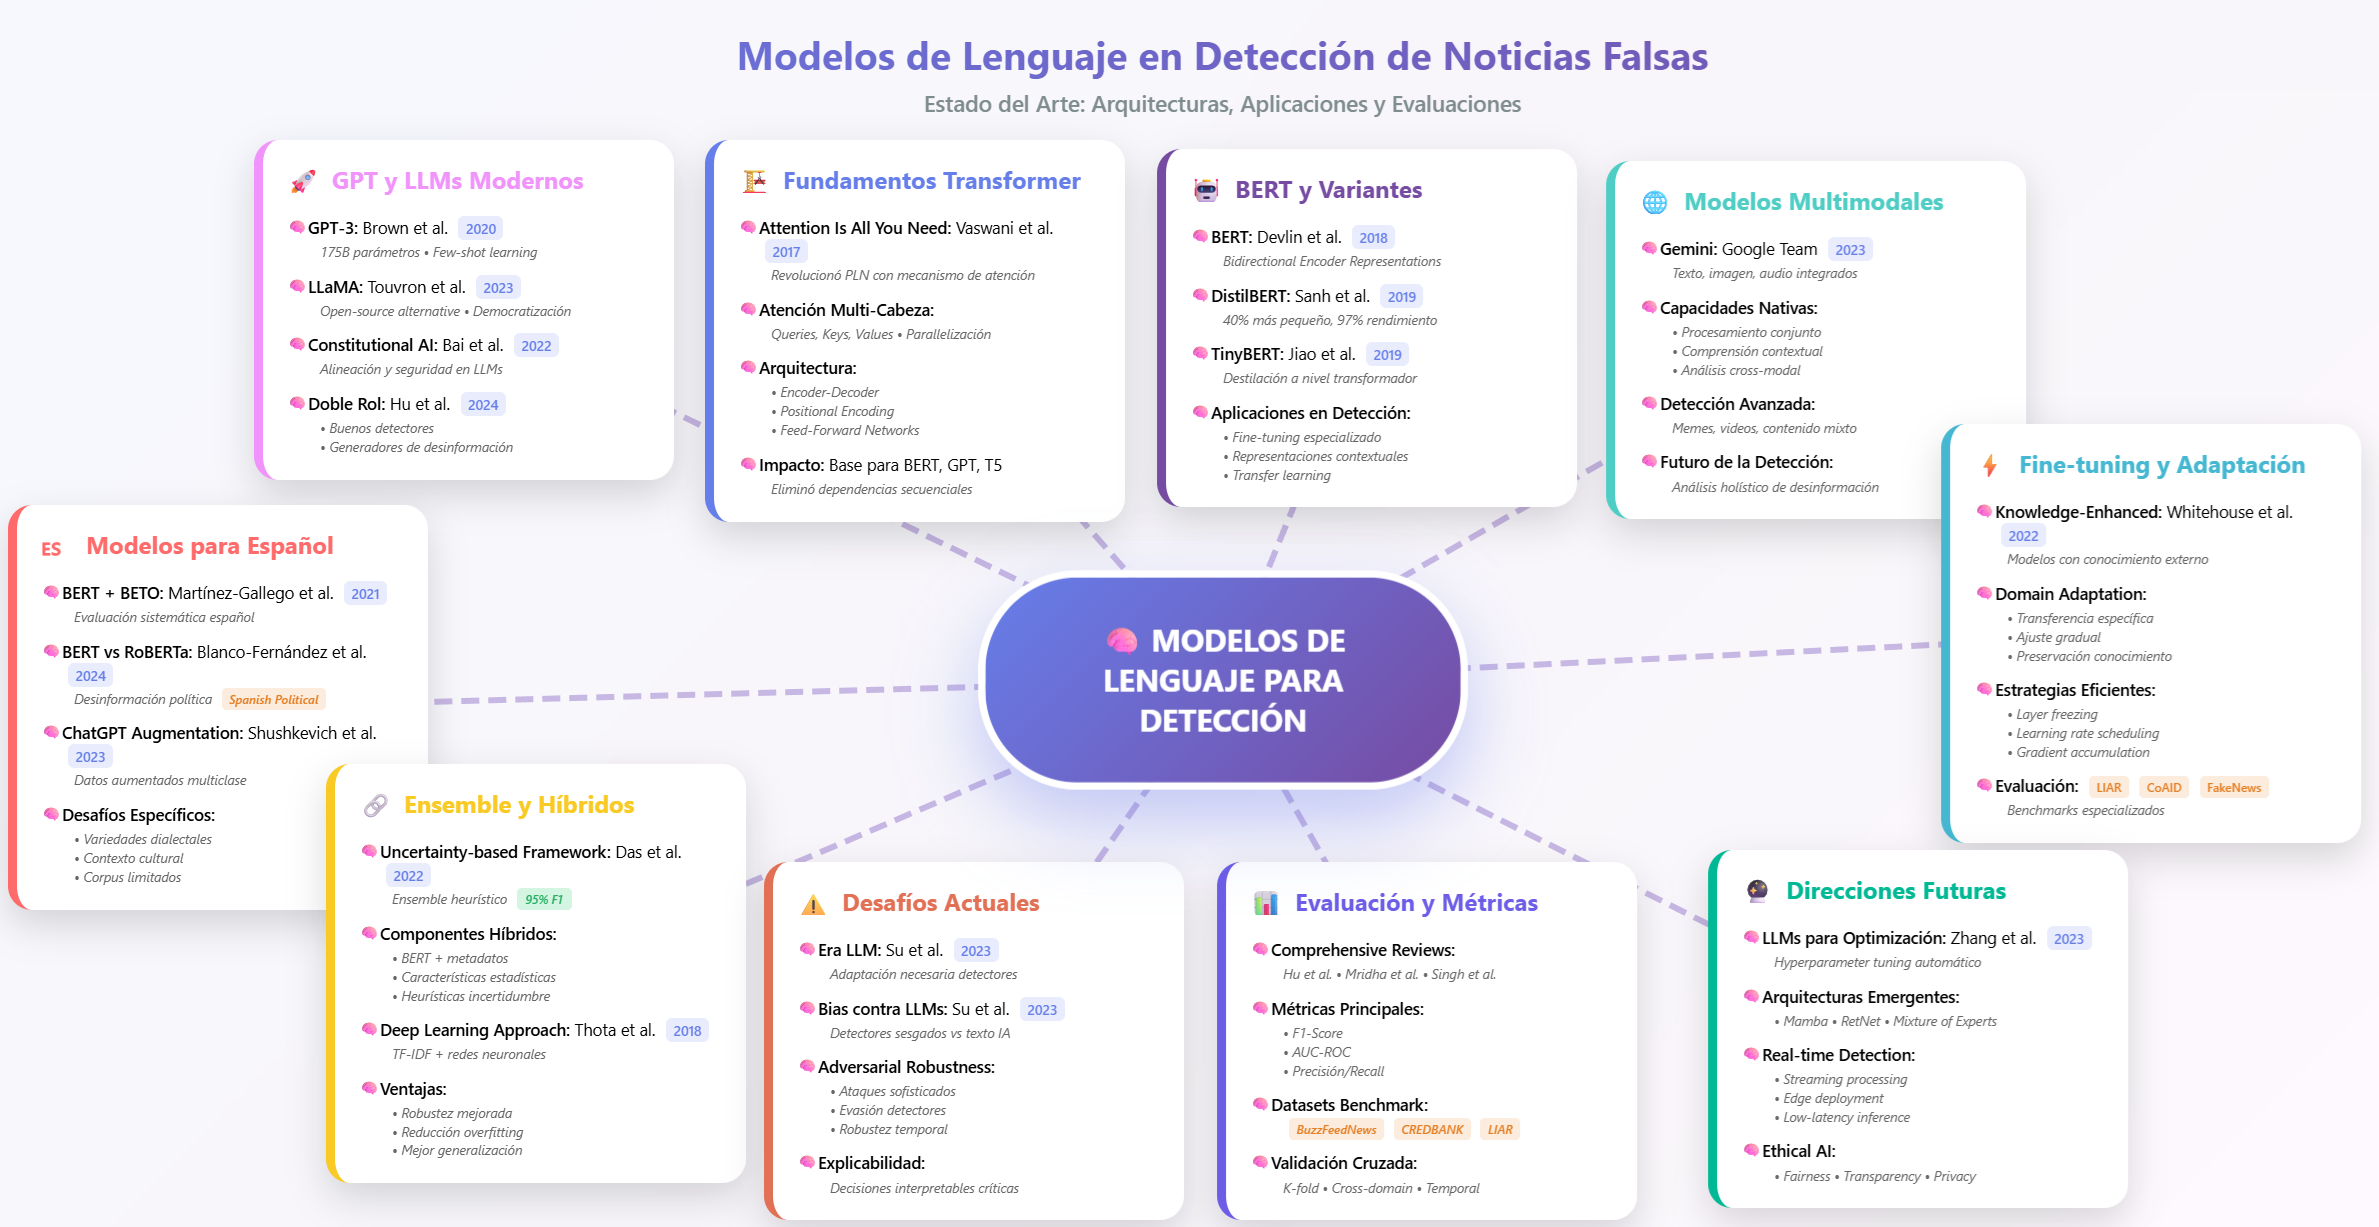
\includegraphics[width=\textwidth]{Imagenes/mapaConceptual3.png}
    \caption{Mapa Conceptual 3: Artículos que son revisiones o están relacionados al análisis de contenido y detección de fraude financiero.}
    \label{fig:mapa_conceptual_3}
\end{figure}

\begin{figure}[h!]
    \centering
    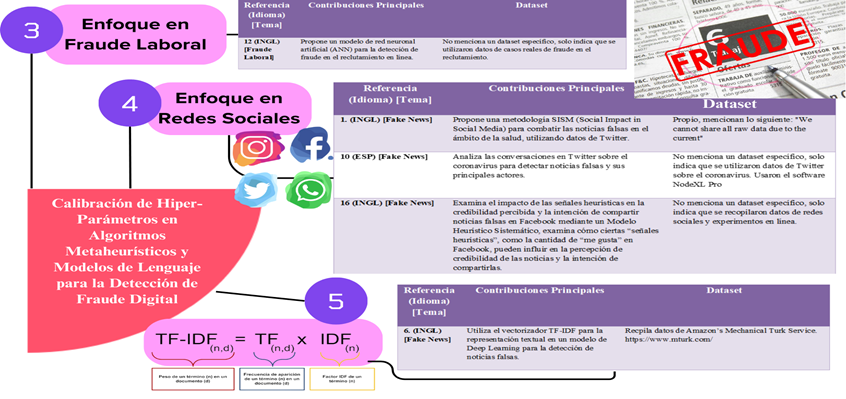
\includegraphics[width=\textwidth]{Imagenes/mapaConceptual4.png}
    \caption{Mapa Conceptual 4: Clasificación de artículos por enfoque metodológico.}
    \label{fig:mapa_conceptual_4}
\end{figure}

\begin{figure}[h!]
    \centering
    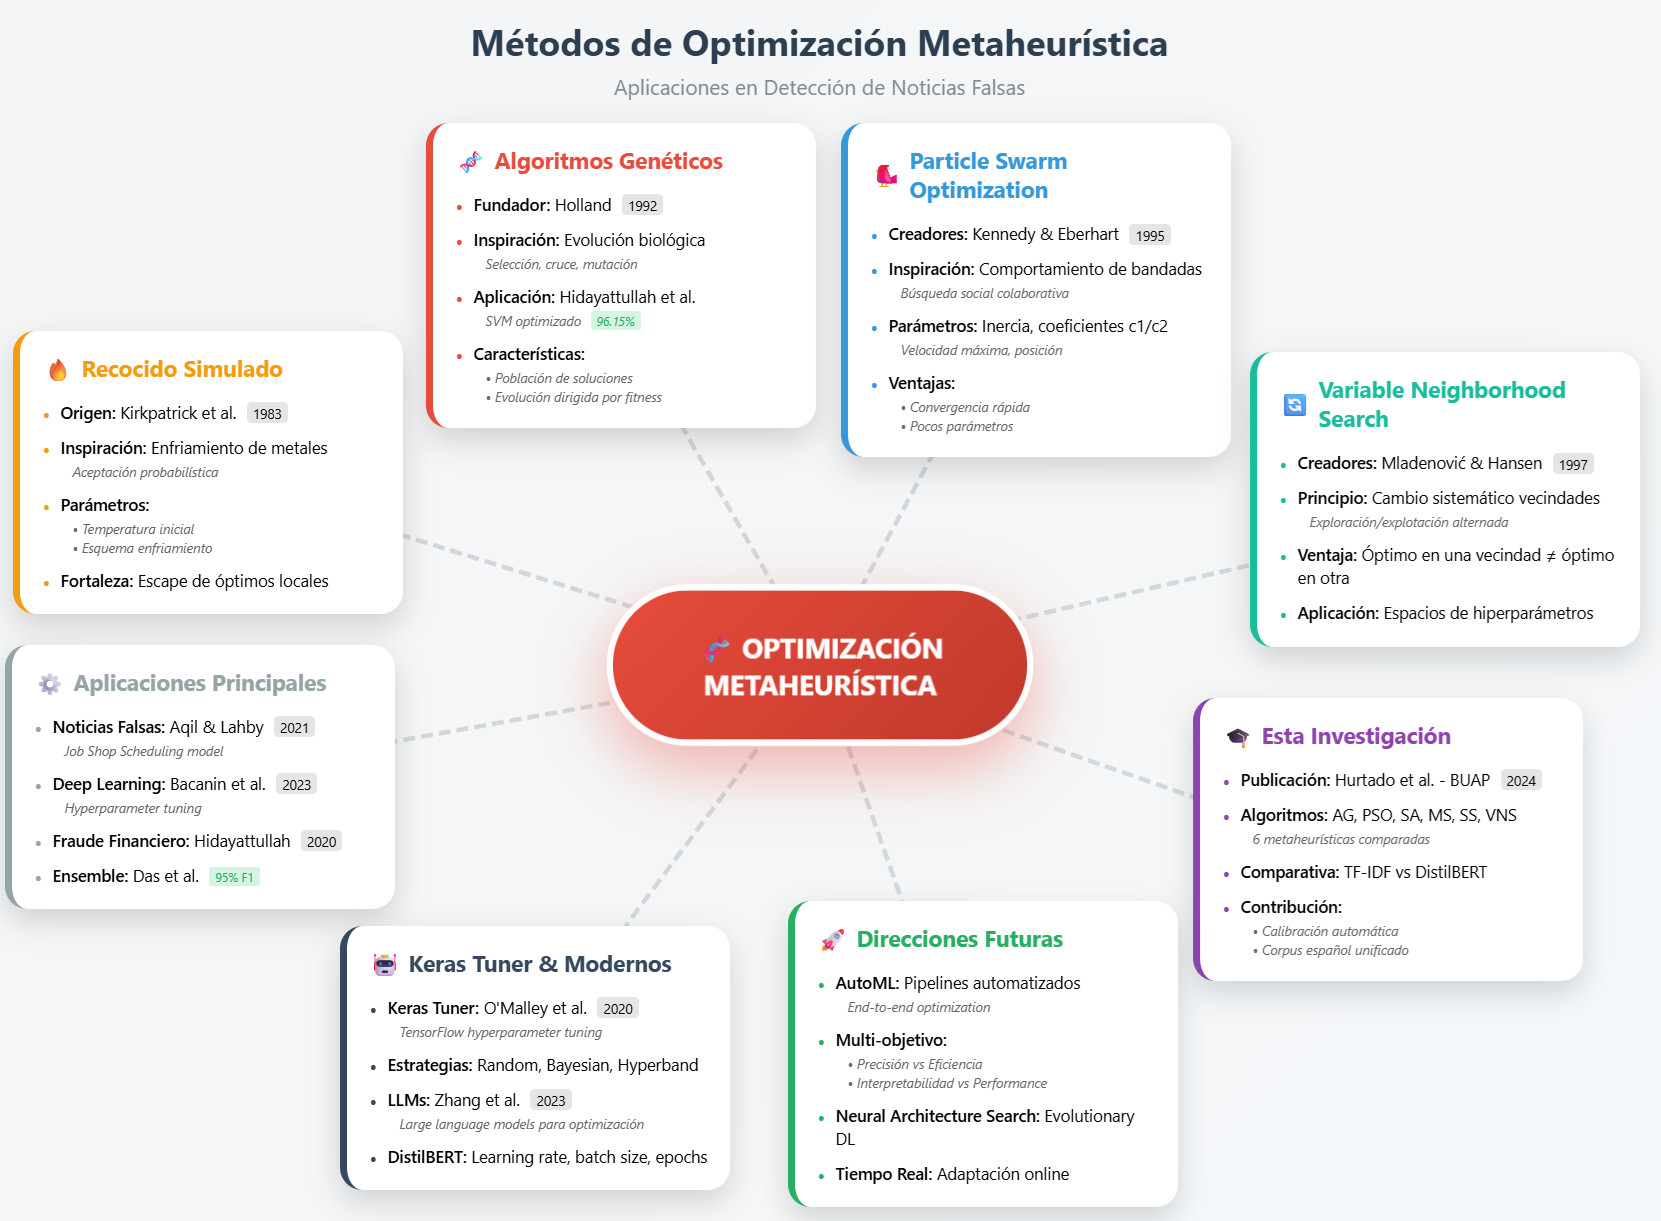
\includegraphics[width=\textwidth]{Imagenes/mapaConceptual5.png}
    \caption{Mapa Conceptual 5: Métodos de optimización y metaheurísticas aplicadas.}
    \label{fig:mapa_conceptual_5}
\end{figure}

\begin{figure}[h!]
    \centering
    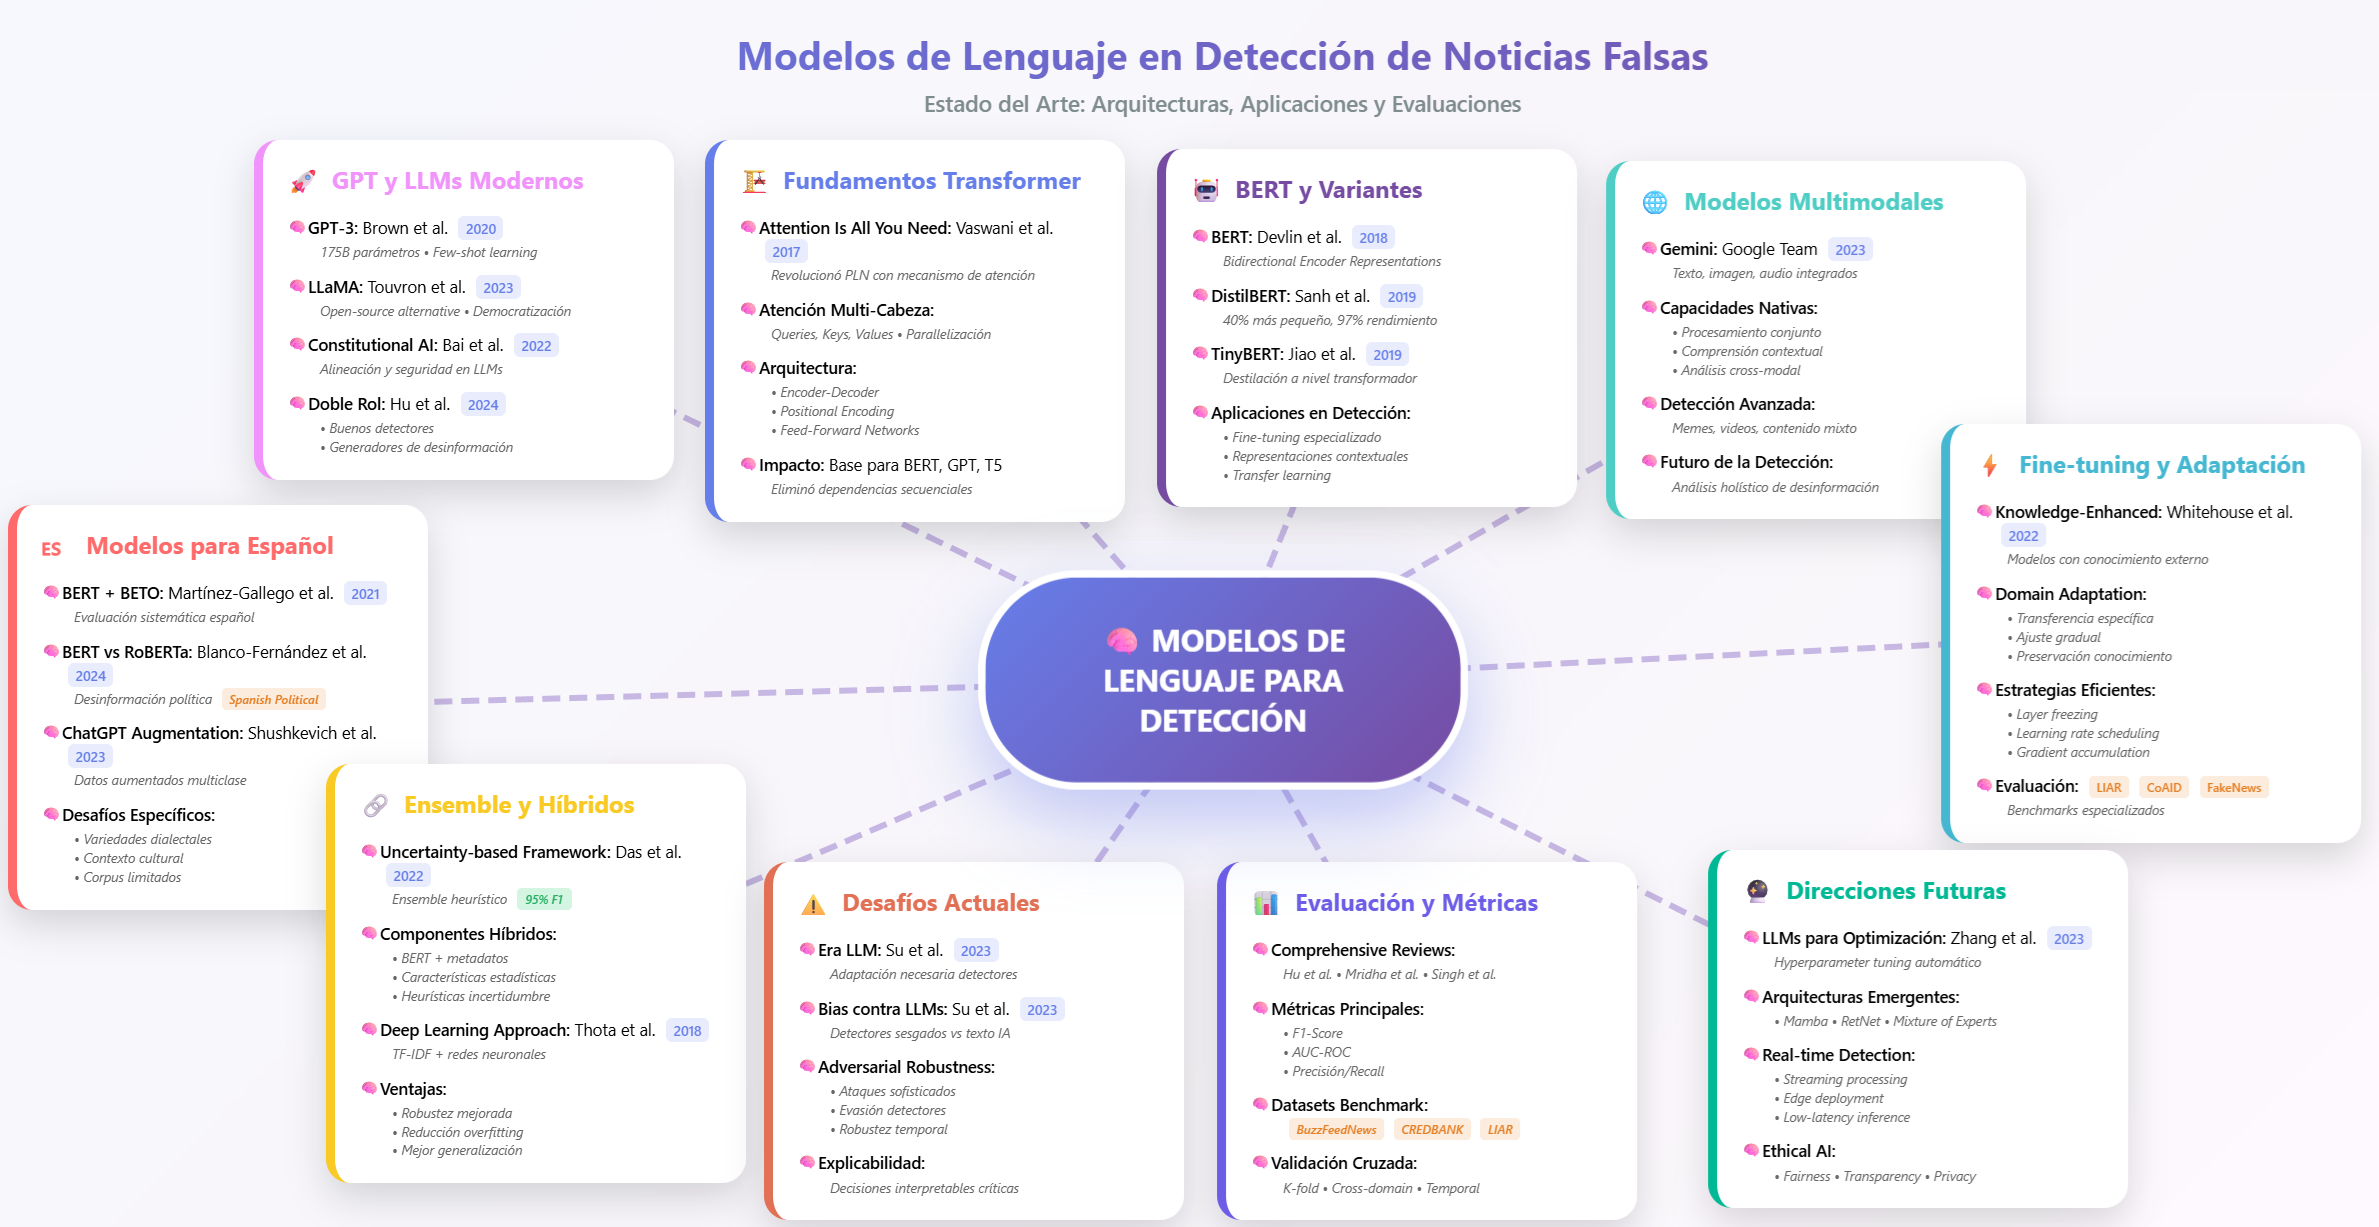
\includegraphics[width=\textwidth]{Imagenes/mapaConceptual6.png}
    \caption{Mapa Conceptual 6: Artículos relacionados que incorporan Modelos de Lenguaje.}
    \label{fig:mapa_conceptual_6}
\end{figure}

\section{Análisis Temático Comprehensivo de la Literatura Relevante}
\label{sec:analisis_tematico}

Más allá de la clasificación taxonómica superficial, resulta fundamental realizar un análisis en profundidad de las contribuciones clave de cada grupo temático identificado, examinando no solo qué se ha hecho, sino cómo se ha hecho, qué resultados se han obtenido, y cuáles son las implicaciones para la planeación y ejecución metodológica de esta tesis. Esta sección proporciona un análisis crítico y detallado de los aportes más significativos de cada categoría de investigación.

\subsection{El Desafío Fundamental de los Datos: Creación y Curación de Corpus en Español}

Uno de los desafíos más fundamentales y persistentes para el Procesamiento del Lenguaje Natural en español es la notable escasez de conjuntos de datos etiquetados de alta calidad a gran escala, especialmente en comparación con los abundantes recursos disponibles en inglés. Esta disparidad en recursos no es meramente cuantitativa, sino que refleja diferencias cualitativas en metodologías de construcción, criterios de calidad, y marcos de evaluación que han limitado históricamente el desarrollo de sistemas de PLN para español.

La creación y curación sistemática de corpus especializados constituye, por tanto, una línea de investigación fundamental que requiere no solo expertise técnico sino también comprensión profunda de las particularidades lingüísticas y culturales del español. El trabajo pionero de Fin de Maestría de Zules Acosta \cite{acosta2019construccion} fue uno de los pioneros más influyentes en este ámbito específico, centrándose meticulosamente en la creación de un conjunto de datos comprensivo de 598 noticias en castellano. Su investigación trasciende la mera recolección de datos para enfocarse profundamente en la importancia crítica de la \textit{ingeniería de características} para seleccionar estrategias óptimas de extracción que permitan a los modelos de aprendizaje automático clasificar eficazmente la veracidad del contenido. El trabajo incluye un análisis detallado de métricas de calidad, procedimientos de validación inter-anotador, y metodologías para manejar ambigüedad en el etiquetado de contenido borderline.

Por otro lado, el trabajo metodológicamente robusto de Posadas-Durán et al. \cite{posadas2019detection} introdujo el influyente \textit{Spanish Fake News Corpus} (con 971 noticias cuidadosamente seleccionadas), estableciéndose como un recurso fundamental para analizar y detectar información engañosa mediante métodos innovadores basados en el estilo de la escritura y características estilométricas avanzadas. Este corpus ha sido fundamental en competencias internacionales como IberLEF, donde se han evaluado sistemáticamente diversas metodologías para el español \cite{gomez2021overview}, incluyendo el análisis especializado de agresividad y noticias falsas en el español de México \cite{aragon2020overview}. La contribución incluye anotaciones de características lingüísticas profundas como complejidad sintáctica, diversidad léxica, y patrones discursivos específicos.

Más recientemente, se han publicado corpus de escala considerablemente mayor que han resultado cruciales para el avance del campo y específicamente para esta tesis. Tretiakov et al. \cite{tretiakov2022detection} aportaron un conjunto de datos significativamente expandido con 1,958 noticias falsas en español, incorporando metadatos enriquecidos sobre fuentes, fechas de publicación, y categorías temáticas. Paralelamente, el trabajo de gran escala de Blanco-Fernández et al. \cite{blanco2024enhancing} introdujo el ambicioso \textit{Spanish Political Fake News Dataset}. Este último recurso, con más de 57,000 noticias meticulosamente recolectadas y etiquetadas, representa uno de los mayores y más comprehensivos recursos disponibles para investigación en español y constituye la fuente principal de datos para esta tesis. La unificación metodológica de estos cuatro corpus diversos constituye el fundamento empírico sólido de este trabajo de investigación.

\subsection{Revolución de los Modelos de Lenguaje y Arquitecturas Transformer}

La arquitectura Transformer, introducida revolucionariamente por Vaswani et al. \cite{vaswani2017attention}, transformó completamente el panorama del PLN con su mecanismo de atención multi-cabeza innovador que permite el procesamiento paralelo eficiente y la captura de dependencias a largo plazo. Este trabajo fundamental estableció las bases teóricas y prácticas para una nueva generación de modelos como BERT \cite{devlin2018bert}, que introdujo el concepto paradigmático de pre-entrenamiento bidireccional, permitiendo a los modelos capturar contexto tanto precedente como subsecuente simultáneamente.

Las variantes optimizadas como DistilBERT \cite{sanh2019distilbert} y TinyBERT \cite{jiao2019tinybert} han demostrado que es posible mantener capacidades semánticas sofisticadas mientras se reduce dramáticamente el costo computacional, haciendo viable la implementación de sistemas de detección en dispositivos con recursos limitados y aplicaciones en tiempo real. Estas innovaciones en eficiencia son particularmente relevantes para implementaciones prácticas de sistemas de detección que deben operar bajo restricciones de latencia y recursos.

El paradigma de los Grandes Modelos de Lenguaje (LLMs) se consolidó definitivamente con GPT-3 \cite{brown2020language}, que demostró capacidades emergentes extraordinarias de few-shot learning y razonamiento en contexto que revolucionaron las expectativas sobre lo que los modelos de lenguaje pueden lograr. Trabajos más recientes como LLaMA \cite{touvron2023llama} han democratizado significativamente el acceso a modelos de gran escala mediante arquitecturas más eficientes y políticas de licenciamiento abierto, mientras que Gemini \cite{gemini2023family} ha avanzado hacia capacidades multimodales que integran texto, imágenes, y otros tipos de información. La investigación en IA Constitucional \cite{bai2022constitutional} ha abordado proactivamente los desafíos críticos de alineación y seguridad de estos sistemas poderosos.

Para el español específicamente, Martínez-Gallego et al. \cite{martinez2021fake} realizaron una exploración sistemática y comprehensiva de la aplicación de BERT y BETO, demostrando empíricamente las ventajas de modelos especializados lingüísticamente. Paralelamente, Blanco-Fernández et al. \cite{blanco2024enhancing} llevaron a cabo comparaciones detalladas entre BERT y RoBERTa para la detección de desinformación, proporcionando evidencia empírica sobre las ventajas específicas de diferentes arquitecturas transformer para este dominio.

La investigación sobre el rol dual de los LLMs \cite{hu2024bad, su2023adapting, su2023fake} ha revelado tanto oportunidades extraordinarias como desafíos significativos en su aplicación para la detección de noticias falsas, incluyendo cuestiones de sesgo, robustez, y generalización que requieren consideración cuidadosa en implementaciones prácticas.

\subsection{Optimización y Metaheurísticas en la Detección: Enfoques Innovadores}

Los algoritmos metaheurísticos han demostrado ser herramientas excepcionalmente valiosas para abordar problemas complejos de optimización en la detección de noticias falsas, proporcionando soluciones elegantes a desafíos que tradicionalmente han sido abordados mediante métodos menos sofisticados. Aqil y Lahby \cite{aqil2021modeling} desarrollaron una formulación innovadora que modela la detección como un problema de scheduling complejo, aplicando algoritmos genéticos, optimización por enjambre de partículas, y otras metaheurísticas para optimizar el pipeline completo de procesamiento.

La calibración de hiperparámetros \cite{bacanin2023benefits, hurtado2024calibracion} ha emergido como una aplicación crítica donde las metaheurísticas superan consistentemente a los métodos tradicionales de grid search y random search, especialmente en espacios de alta dimensionalidad donde la búsqueda exhaustiva es computacionalmente prohibitiva. Estos enfoques han demostrado capacidad superior para navegar paisajes de optimización complejos y multimodales característicos del ajuste de modelos profundos.

El enfoque innovador de ensemble con marcos heurísticos \cite{das2022heuristic} ha mostrado resultados especialmente prometedores al combinar múltiples modelos especializados con información estadística adicional, creando sistemas que pueden manejar incertidumbre de manera más sofisticada que enfoques de clasificación tradicionales. Yildirim \cite{yildirim2023novel} propuso un enfoque híbrido multi-thread particularmente avanzado que optimiza simultáneamente tanto la selección de características como los parámetros del modelo, demostrando el potencial de optimización coordinada en múltiples dimensiones del problema.

La aplicación de PSO para la detección de reseñas falsas \cite{deshai2023unmasking} demuestra convincentemente la versatilidad y transferabilidad de estas técnicas más allá del dominio específico de noticias, sugiriendo principios generalizables para la detección de contenido desinformativo en múltiples contextos.

\subsection{Aplicación de Metaheurísticas por Tipo de Detección}
\label{subsec:metaheuristicas_por_tipo}

La literatura revisada revela patrones específicos y sistemáticos en la aplicación de algoritmos metaheurísticos según el tipo de detección, el dominio del problema, y las características específicas de los datos involucrados. Esta taxonomía detallada proporciona insights valiosos para la selección informada de técnicas de optimización para diferentes contextos de aplicación.

\begin{table}[htbp]
\centering
\adjustbox{width=\textwidth,center}{%
\small
\begin{tabular}{|l|l|l|l|c|}
\hline
\rowcolor{UAMPurple!20}
\textbf{Tipo de Detección} & \textbf{Metaheurística Empleada} & \textbf{Aplicación Específica} & \textbf{Autores} & \textbf{Ref.} \\
\hline
\begin{tabular}[t]{@{}l@{}}Detección de\\Noticias Falsas\end{tabular} & \begin{tabular}[t]{@{}l@{}}Algoritmo Genético (GA),\\Colonia de Abejas (ABC),\\Búsqueda Iterativa (IG)\end{tabular} & \begin{tabular}[t]{@{}l@{}}Planificación de tareas\\para procesamiento\\de documentos\end{tabular} & Aqil, S. \& Lahby, M. & \cite{aqil2021modeling} \\
\hline
\begin{tabular}[t]{@{}l@{}}Detección de\\Reseñas Falsas\end{tabular} & \begin{tabular}[t]{@{}l@{}}Optimización por\\Enjambre de Partículas\\Adaptativo (PSO)\end{tabular} & \begin{tabular}[t]{@{}l@{}}Optimización de\\hiperparámetros en\\redes CNN\end{tabular} & \begin{tabular}[t]{@{}l@{}}Deshai, N. \&\\Rao, B. B.\end{tabular} & \cite{deshai2023unmasking} \\
\hline
\begin{tabular}[t]{@{}l@{}}Fraude Financiero\\y de Estados\\Financieros\end{tabular} & \begin{tabular}[t]{@{}l@{}}Algoritmos Genéticos,\\Optimización por\\Enjambre de Partículas,\\Recocido Simulado\end{tabular} & \begin{tabular}[t]{@{}l@{}}Selección de características\\y optimización de\\clasificadores SVM\end{tabular} & \begin{tabular}[t]{@{}l@{}}Hidayattullah, S.\\et al.\end{tabular} & \cite{hidayattullah2020financial} \\
\hline
\begin{tabular}[t]{@{}l@{}}Predicción de\\Dificultades\\Financieras\end{tabular} & \begin{tabular}[t]{@{}l@{}}Optimización Bayesiana\\con Procesos\\Gaussianos\end{tabular} & \begin{tabular}[t]{@{}l@{}}Calibración de\\hiperparámetros\\en modelos GPR\end{tabular} & \begin{tabular}[t]{@{}l@{}}Horak, J. \&\\Sabek, A.\end{tabular} & \cite{horak2023gaussian} \\
\hline
\begin{tabular}[t]{@{}l@{}}Detección de\\Fraude Laboral\end{tabular} & \begin{tabular}[t]{@{}l@{}}Redes Neuronales\\Artificiales (ANN)\end{tabular} & \begin{tabular}[t]{@{}l@{}}Clasificación de\\ofertas de empleo\\fraudulentas\end{tabular} & \begin{tabular}[t]{@{}l@{}}Nasser, I. M.\\et al.\end{tabular} & \cite{nasser2021online} \\
\hline
\begin{tabular}[t]{@{}l@{}}Optimización de\\Modelos de Energía\end{tabular} & \begin{tabular}[t]{@{}l@{}}Algoritmo Genético\\Binario, PSO, Recocido\\Simulado, Búsqueda\\Armónica\end{tabular} & \begin{tabular}[t]{@{}l@{}}Ajuste de hiperparámetros\\en modelos LSTM\\para predicción energética\end{tabular} & \begin{tabular}[t]{@{}l@{}}Bacanin, N.\\et al.\end{tabular} & \cite{bacanin2023benefits} \\
\hline
\begin{tabular}[t]{@{}l@{}}Detección Multimodal\\de Noticias Falsas\end{tabular} & \begin{tabular}[t]{@{}l@{}}Enfoque Híbrido\\Multi-hilo con\\Metaheurísticas\end{tabular} & \begin{tabular}[t]{@{}l@{}}Optimización paralela\\de características\\textuales y visuales\end{tabular} & Yildirim, G. & \cite{yildirim2023novel} \\
\hline
\begin{tabular}[t]{@{}l@{}}Selección de\\Características\\para Fake News\end{tabular} & \begin{tabular}[t]{@{}l@{}}K-Means combinado\\con Support Vector\\Machine (SVM)\end{tabular} & \begin{tabular}[t]{@{}l@{}}Reducción de\\dimensionalidad\\y mejora de precisión\end{tabular} & \begin{tabular}[t]{@{}l@{}}Yazdi, K. M.\\et al.\end{tabular} & \cite{yazdi2020improving} \\
\hline
\begin{tabular}[t]{@{}l@{}}Framework de\\Incertidumbre\\para Fake News\end{tabular} & \begin{tabular}[t]{@{}l@{}}Enfoque Heurístico\\basado en Ensemble\end{tabular} & \begin{tabular}[t]{@{}l@{}}Manejo de incertidumbre\\en clasificación de\\tweets y artículos\end{tabular} & \begin{tabular}[t]{@{}l@{}}Das, S. D.\\et al.\end{tabular} & \cite{das2022heuristic} \\
\hline
\begin{tabular}[t]{@{}l@{}}Optimización de\\Dominación Total\\en Redes Sociales\end{tabular} & \begin{tabular}[t]{@{}l@{}}Búsqueda en\\Vecindades Variables\\(VNS)\end{tabular} & \begin{tabular}[t]{@{}l@{}}Propagación de\\información en\\redes sociales\end{tabular} & \begin{tabular}[t]{@{}l@{}}Kapunac, S.\\et al.\end{tabular} & \cite{kapunac2023variable} \\
\hline
\begin{tabular}[t]{@{}l@{}}Estimación de\\Esfuerzo en\\Proyectos\end{tabular} & \begin{tabular}[t]{@{}l@{}}Ensemble con\\Metaheurísticas\\para Pesos\end{tabular} & \begin{tabular}[t]{@{}l@{}}Optimización de\\hiperparámetros\\y pesos de ensemble\end{tabular} & \begin{tabular}[t]{@{}l@{}}Yasmin, A.\\et al.\end{tabular} & \cite{yasmin2024ensemble} \\
\hline
\end{tabular}
}
\caption{Aplicación de metaheurísticas por tipo de detección en la literatura revisada.}
\label{tab:metaheuristicas_deteccion}
\end{table}

\subsubsection{Patrones Identificados por Dominio}

Del análisis sistemático de la literatura se identifican tres patrones principales y claramente diferenciados en la aplicación de metaheurísticas:

\paragraph{Detección de Contenido Textual}
Para la detección de noticias falsas y contenido textual fraudulento, predominan los enfoques que combinan estratégicamente:
\begin{itemize}
    \item \textbf{Algoritmos Genéticos}: Utilizados principalmente para selección de características en espacios de alta dimensionalidad y optimización de arquitecturas de modelos complejos \cite{aqil2021modeling, hidayattullah2020financial}
    \item \textbf{PSO Adaptativo}: Especialmente efectivo para la calibración de hiperparámetros en redes neuronales complejas donde el espacio de búsqueda es continuo y las evaluaciones son costosas \cite{deshai2023unmasking, bacanin2023benefits}
    \item \textbf{Enfoques Híbridos}: Combinación sinérgica de múltiples metaheurísticas para diferentes aspectos del pipeline de detección, optimizando simultáneamente múltiples objetivos \cite{yildirim2023novel}
\end{itemize}

\paragraph{Optimización de Modelos de Aprendizaje Profundo}
En aplicaciones que involucran modelos de aprendizaje profundo y arquitecturas complejas, se observa una preferencia marcada por:
\begin{itemize}
    \item \textbf{Recocido Simulado}: Particularmente efectivo para escapar de óptimos locales en espacios de hiperparámetros complejos y multimodales \cite{bacanin2023benefits}
    \item \textbf{Optimización Bayesiana}: Para calibración eficiente en modelos probabilísticos donde se requiere balance entre exploración y explotación \cite{horak2023gaussian}
    \item \textbf{Búsqueda en Vecindades Variables}: Para exploración sistemática de configuraciones de red mediante cambio de estructuras de vecindad \cite{kapunac2023variable}
\end{itemize}

\paragraph{Sistemas de Detección en Tiempo Real}
Para aplicaciones que requieren procesamiento en tiempo real y alta throughput, las metaheurísticas se enfocan estratégicamente en:
\begin{itemize}
    \item \textbf{Algoritmos de Planificación}: Como IG (Iterated Greedy) para optimización de tareas de procesamiento con restricciones temporales \cite{aqil2021modeling}
    \item \textbf{Métodos Ensemble}: Con optimización de pesos mediante metaheurísticas para combinar múltiples detectores especializados \cite{das2022heuristic, yasmin2024ensemble}
    \item \textbf{Enfoques Multi-hilo}: Para paralelización eficiente de la optimización en sistemas multimodales que procesan múltiples tipos de información simultáneamente \cite{yildirim2023novel}
\end{itemize}

Esta taxonomía detallada revela que la elección de la metaheurística está fuertemente influenciada por factores como el tipo de modelo subyacente, las características del conjunto de datos, los requisitos de rendimiento temporal del sistema de detección, y las restricciones computacionales específicas del entorno de implementación.

\subsection{Perspectivas Interdisciplinarias y Análisis Social}

La comprensión profunda del fenómeno de las noticias falsas requiere necesariamente un enfoque interdisciplinario sofisticado que combine aspectos técnicos avanzados con análisis social, psicológico, y cultural. Los aspectos puramente técnicos, aunque fundamentales, son insuficientes para abordar completamente la complejidad multifacética de la desinformación moderna.

Ali et al. \cite{ali2021fake, ali2020posttruth} han investigado sistemáticamente cómo las heurísticas cognitivas humanas, incluyendo señales de popularidad social como el número de "me gusta" y compartidos, influyen significativamente en la percepción de credibilidad de contenido digital. Su trabajo sobre el procesamiento heurístico durante eventos políticos específicos, particularmente las elecciones presidenciales de 2016 en Estados Unidos, proporciona insights valiosos y empíricamente fundamentados sobre la psicología de la desinformación y los mecanismos cognitivos que hacen a las personas susceptibles a información falsa.

El análisis detallado del rol de los medios de comunicación tradicionales \cite{carcamo2021fake, perez2020fake} ha revelado patrones culturales importantes en cómo diferentes países y culturas abordan, conceptualizan, y responden al problema de la desinformación. Estos estudios transculturales proporcionan evidencia empírica sobre la importancia de considerar factores culturales en el diseño de sistemas de detección automatizada.

Pulido et al. \cite{pulido2020new} propusieron el marco innovador SISM (Social Impact in Social Media) para combatir específicamente la desinformación en el dominio de la salud, un área particularmente crítica durante pandemias y crisis de salud pública donde la desinformación puede tener consecuencias directas sobre la vida y muerte de las personas.

\subsection{Detección de Fraude: Extensión Más Allá de las Noticias}

La investigación en detección de fraude ha diversificado significativamente sus aplicaciones, extendiéndose más allá del dominio específico de noticias falsas hacia otros contextos de fraude digital que presentan características similares pero requieren adaptaciones específicas.

En el ámbito laboral específicamente, Nasser et al. \cite{nasser2021online} desarrollaron sistemas basados en redes neuronales artificiales para detectar ofertas de trabajo fraudulentas, demostrando que las técnicas desarrolladas para detección de noticias falsas pueden transferirse efectivamente a otros dominios textuales. Paralelamente, Alvarez \cite{alvarez2021fraude} analizó comprehensivamente las nuevas modalidades de fraude laboral en la era digital latinoamericana, proporcionando contexto regional importante para entender las manifestaciones específicas del fraude en diferentes contextos socioeconómicos.

En el sector financiero, la investigación de Hidayattullah et al. \cite{hidayattullah2020financial} demostró empíricamente la efectividad de combinar aprendizaje automático con optimización metaheurística para detectar fraudes en estados financieros, estableciendo precedentes metodológicos importantes. Cao et al. \cite{cao2020corporate} establecieron conexiones innovadoras entre indicadores de empleo corporativo y riesgo de fraude, proporcionando herramientas valiosas para auditores y reguladores financieros.

\section{Síntesis y Perspectivas Futuras}
\label{sec:sintesis_perspectivas}

La revisión comprehensiva y sistemática de la literatura revela una evolución clara y acelerada en las aproximaciones para la detección de noticias falsas y fraude digital. Desde los primeros enfoques relativamente simples basados en características lingüísticas superficiales hasta los modernos sistemas sofisticados basados en transformers y LLMs, el campo ha experimentado avances extraordinarios en términos de precisión, escalabilidad, y aplicabilidad práctica.

Los desafíos principales identificados a través de esta revisión incluyen: (1) la necesidad imperativa de mayor cantidad de datos etiquetados de alta calidad en español, (2) la adaptación cultural y lingüística de modelos a contextos específicos del mundo hispanohablante, (3) la optimización eficiente de hiperparámetros en modelos cada vez más complejos, y (4) la integración inteligente de información multimodal y conocimiento externo estructurado.

Esta tesis contribuye especialmente a los puntos (1) y (3) mediante la unificación metodológica de corpus existentes en una escala sin precedentes y la aplicación sistemática de técnicas metaheurísticas avanzadas para la optimización de modelos de detección de última generación.

La organización temática comprehensiva presentada en este capítulo proporciona un marco conceptual robusto para entender las diferentes dimensiones del problema de detección de desinformación y justifica empíricamente la aproximación metodológica híbrida adoptada en esta investigación, que combina inteligentemente modelos de lenguaje state-of-the-art con técnicas de optimización metaheurística para lograr rendimiento superior en la detección de contenido desinformativo en español.

Las perspectivas futuras incluyen la evolución hacia sistemas adaptativos que puedan evolucionar con las técnicas de desinformación cambiantes, la integración de conocimiento factual en tiempo real, y el desarrollo de marcos éticos para el despliegue responsable de tecnologías de detección automatizada.